\documentclass{LIKE}

\definecolor{MainGreen}{RGB}{22, 160, 133}
\definecolor{MainPurple}{RGB}{142, 68, 173}
\definecolor{MainYellow}{RGB}{211, 84, 0}
\definecolor{MainBlue}{RGB}{41, 128, 185}
\definecolor{MainRed}{RGB}{192, 57, 43}
\definecolor{MainBlack}{RGB}{44, 62, 80}

\begin{document}

\vfill
\begin{tikzpicture}[remember picture, overlay]
    \node[anchor=north west, inner sep=0] at (current page.north west) {%
        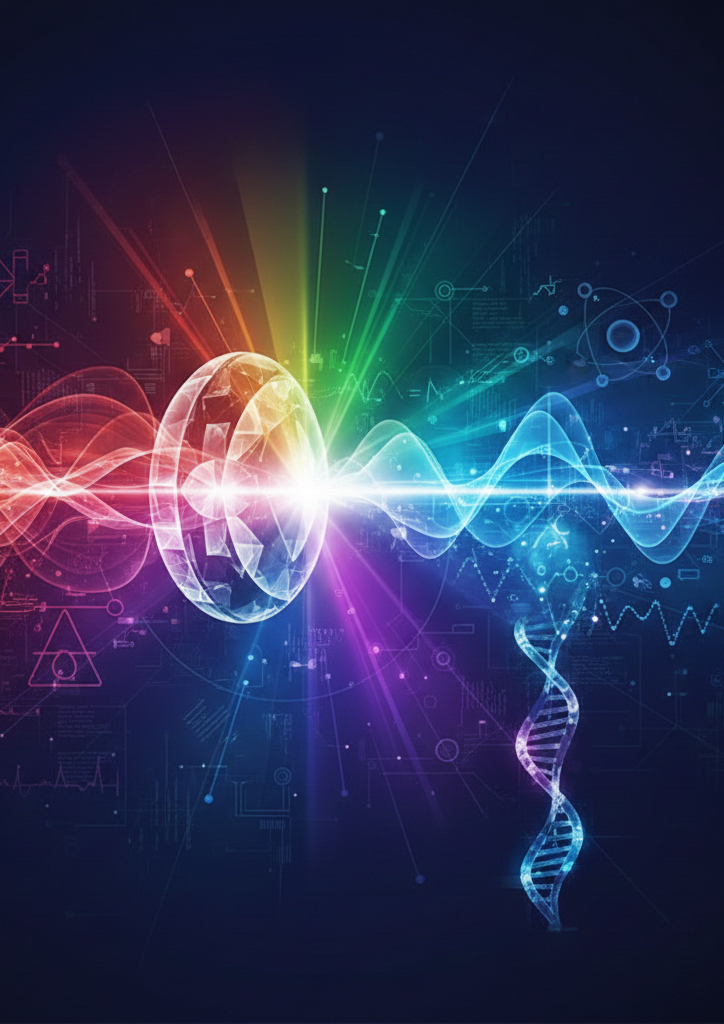
\includegraphics[width=\paperwidth, height=\paperheight]{asset/cover3.png} 
    };

    \fill[JungleGreen] 
        (current page.north east) rectangle ++(-8.0cm, -12.0cm);
    
    %\coordinate (topright) at ([xshift=-2cm, yshift=-5cm]current page.north east);
    \fill[white] 
        ([xshift=-2cm, yshift=-5cm]current page.north east) rectangle ++(-6.0cm, -7.0cm); 

    % “大学物理”大字
    \node[font=\fontsize{64}{64}\selectfont\bfseries, anchor=center] 
        at ([xshift=-5cm, yshift=-6.8cm]current page.north east) {大学};
    \node[font=\fontsize{64}{64}\selectfont\bfseries, anchor=center] 
        at ([xshift=-5cm, yshift=-9.3cm]current page.north east) {物理};

    \fill[brown!90!black] 
        ([xshift=-2cm, yshift=-12cm]current page.north east) rectangle ++(-6.0cm, -2.5cm);
        
    \node[font=\fontsize{18}{22}\selectfont\sffamily\bfseries, Gray, anchor=center] 
        at ([xshift=-5cm, yshift=-11.2cm]current page.north east) {必修~3};
    \node[font=\fontsize{24}{24}\selectfont\bfseries, black, anchor=center] 
        at ([xshift=-5cm, yshift=-12.75cm]current page.north east) {热学~光学};
    \node[font=\fontsize{24}{24}\selectfont\bfseries, black, anchor=center] 
        at ([xshift=-5cm, yshift=-13.75cm]current page.north east) {近代物理};

    \node[font=\fontsize{12}{14}\selectfont, text=black, anchor=center] 
        at ([xshift=-5cm, yshift=-2.8cm]current page.north east) {大~学~课~程~自~编~讲~义};
        
    \node[font=\fontsize{14}{14}\selectfont\sffamily\bfseries, text=white, anchor=center] 
        at ([xshift=3cm, yshift=2cm]current page.south west) {张云翼~~编};
\end{tikzpicture}

\newpage

\colorlet{maincolor}{MainYellow}
\colorlet{sidecolor}{MainYellow!50}

\setcounter{part}{3}

\setcounter{chapter}{12}

\part{热学}

\chapter{气体动理论}
\setcounter{example_counter}{1}

\section{理想气体}

\subsection{热学研究对象}

\vspace{-0.5em}

\subsubsection{系统}

热学的研究对象是大量微观粒子（分子、原子）构成的体积有限的物体，称为\textbf{热力学系统}，简称\textbf{系统}。

\note{在热学中，不区分物质是由分子、原子还是离子构成的，构成物质的最小微粒统称为分子。}

%\begin{itemize}
%    \item 孤立系统：与外界没有任何相互作用，既无能量、也无物质交换
%    \item 封闭系统：与外界有能量、但无物质交换
%    \item 开放系统：与外界既有能量又有物质交换
%\end{itemize}

\subsubsection{气体动理论基本观点}

\noindent
\begin{minipage}{0.73\textwidth}
    \setlength{\parskip}{0.5em}
    \setlength{\parindent}{2em}
    \linespread{1.3}

    \vspace{0.5em}

\begin{itemize}
    \item 宏观物体由大量分子构成，分子之间存在空隙
    \item 分子永不停息地作无规则运动
    \item 分子间有一定相互作用力
\end{itemize}
    
\end{minipage}
\hfill
\begin{minipage}{0.25\textwidth}
    \centering 
\includegraphics[width=\textwidth]{asset/ch6/T1.png}
\end{minipage}

\subsubsection{理想气体的微观假设}

\begin{itemize}
    \item 忽略分子本身的形状和大小
    \item 不考虑分子间除碰撞外的其他相互作用
    \item 分子行为服从牛顿运动定律，所有碰撞均为弹性碰撞
\end{itemize}

\subsection{理想气体物态方程}

\begin{itemize}
    \item 形式1：$pV=\nu RT$，其中$\nu$表示物质的量，气体常数$R=\SI{8.314}{J/(mol\cdot K)}$
    \item 形式2：$p=nkT$，其中$n=\dfrac{N}{V}$表示分子数密度，玻尔兹曼常数$k=\SI{1.38e-23}{J/K}$
\end{itemize}

\begin{formula}
    \centering $pV=\nu RT$ 或 $p=nkT$
\end{formula}

\note{物质的量$\nu=\dfrac{m}{M}$，阿伏伽德罗常数$N_A=\SI{6.02e23}{mol^{-1}}$，玻尔兹曼常数$k=\dfrac{R}{N_A}$}

\warn{需要特别小心$n,\nu$的含义，两个常数的值不需要记忆。}

在热学中，温度$T$都要采用热力学温标，它与摄氏温标$t$的关系为

\begin{formula}
    \centering $T=t+273.15$
\end{formula}

\note{温度是有下限的，热力学第三定律指出，绝对零度（$\SI{0}{K}$）不可达到。}

\begin{example}{理想气体物态方程}
    已知一容器中理想气体在$\SI{0}{\degreeCelsius}$、$\SI{1.0e-2}{atm}$条件下的密度为$\SI{12.4}{g/m^3}$，气体常数取$R=\SI{8.31}{J/(mol\cdot K)}$，求该气体的摩尔质量$M$。
    \tcblower  
    {\fangsong 思路：直接代入理想气体状态方程即可，注意各个量的含义和单位。}
    \tcbline
    理想气体状态方程$pV=\nu RT$，已知条件中的密度$\rho=\dfrac{m}{V}$
    
    结合物质的量$\nu=\dfrac{m}{M}$，联立解得$M=\dfrac{\rho RT}{p}$
    
    温度$T=\SI{273.15}{K}$，压强$p=\SI{1e3}{Pa}$，代入求得$M\approx \SI{28.13}{g/mol}$
    \tcbline
    【补充练习】一封闭容器中间有可自由移动的导热活塞，一侧装有$\SI{0.1}{kg}$氢气，另一侧装有一定量氧气。若要使平衡状态下，活塞位于正中间，求应充入氧气的质量。
\end{example}

\subsection{气体的无规则运动}

\subsubsection{分子运动的无规则性}

\begin{itemize}
    \item 气体分子无时无刻不在做无规则运动，达到平衡态时，气体的性质与方向无关
    \item 分子出现在各处的概率相等
    \item 各个方向上的速度分布完全相同，因此各个方向上的平均速度都是零
    \item 各个方向上速率的平方平均值相等，都等于总平均值的$\dfrac{1}{3}$
\end{itemize}

\begin{formula}
    $\overline{v_x}=\overline{v_y}=\overline{v_z}=0,~~~\overline{v_x^2}=\overline{v_y^2}=\overline{v_z^2}=\dfrac{1}{3}\overline{v^2}$
\end{formula}

这里$\overline{v^2}$是取各分子速率平方的平均值，其算术平方根$\sqrt{\overline{v^2}}$称为方均根速率。

\subsubsection{平均碰撞频率与自由程}

若将气体分子视为直径为$d$的球体，推导可得平均碰撞频率$\bar{z}=\sqrt{2}\pi d^2 \bar{v} n$.

平均自由程$\bar{\lambda}$是指一个气体分子在两次碰撞之间运动的平均距离，等于平均速率除以平均碰撞频率。

\begin{formula}
    $\bar{z}=\sqrt{2}\pi d^2 \bar{v} n,~~~\bar{\lambda}=\dfrac{\bar{v}}{\bar{z}}=\dfrac{1}{\sqrt{2}\pi d^2 n}$
\end{formula}

\note{气体分子越大、越密、运动越快，则碰撞频率越大，但平均自由程与运动速率无关。}

结合$p=nkT$，可得$\bar{\lambda}=\dfrac{kT}{\sqrt{2}\pi d^2 p} \propto \dfrac{T}{p}$，与体积$V$无直接关系。

碰撞截面$\sigma=\pi d^2$，则
\begin{formula}
    $\bar{z}=\sqrt{2}\sigma \bar{v} n,~~~\bar{\lambda}=\dfrac{\bar{v}}{\bar{z}}=\dfrac{1}{\sqrt{2}\sigma n}$
\end{formula}

\begin{example}{碰撞频率与自由程}
    一定量理想气体，若温度和体积都变为原来的$2$倍，则平均自由程、平均碰撞频率如何变化？
    \tcblower  
    (1)~根据$\bar{v}=\sqrt{\dfrac{8RT}{\pi M}}$，可知温度变为$2$倍，则平均速率变为原来的$\sqrt{2}$倍

    根据公式$\bar{\lambda}=\dfrac{\bar{v}}{\bar{z}}=\dfrac{1}{\sqrt{2}\pi d^2 n}$，可知平均自由程变为原来的$2$倍。

    (2)~体积变为$2$倍，则分子数密度$n$变为一半，结合$\bar{z}=\sqrt{2}\pi d^2 \bar{v} n$，可知平均碰撞频率变为$\dfrac{\sqrt{2}}{2}$倍。

    \tcbline
    【补充练习】气缸内有一定量的氢气，若温度不变，而压强变为原来的2倍，则平均碰撞频率、平均自由程变为原来的几倍？
\end{example}

\section{温度与压强的微观含义}

\subsection{压强}

\noindent
\begin{minipage}{0.78\textwidth}
    \setlength{\parskip}{0.5em}
    \setlength{\parindent}{2em}
    \linespread{1.3}

气体的压强是由于气体分子持续撞击容器壁而形成的。

记$\overline{\varepsilon_t}$表示气体分子的平均平动动能，$n$表示分子数密度，则理想气体的压强

\begin{formula}
    $p=\dfrac{2}{3}n\overline{\varepsilon_t}$
\end{formula}
    
\end{minipage}
\hfill
\begin{minipage}{0.2\textwidth}
    \centering 
\includegraphics[width=\textwidth]{asset/ch6/T3.png}
\end{minipage}

其中，分子的平均平动动能可用每个分子的质量$m_0$表示为$\overline{\varepsilon_t}=\dfrac{1}{2}m_0\overline{v^2}$.

\subsection{温度}

\subsubsection{热平衡定律}

一个系统的各种性质不随时间改变的状态称为\textbf{平衡态}，热学中的平衡态应理解为动态平衡。

如果物体A和B能分别与物体C的同一状态处于平衡态，则将此时的A和B放到一起，它们也必定处于平衡态，这就是\textbf{热平衡定律}，也称为\textbf{热力学第零定律}。

\subsubsection{温度的微观含义}

\noindent
\begin{minipage}{0.78\textwidth}
    \setlength{\parskip}{0.5em}
    \setlength{\parindent}{2em}
    \linespread{1.3}

两个处于平衡态的系统，应有某个参量是相等的，这个参量就定义为\textbf{温度}。

由$p=\dfrac{2}{3}n\overline{\varepsilon_t}=nkT$，可得温度与分子的平均平动动能成正比。

\begin{formula}
    $\overline{\varepsilon_t}=\dfrac{3}{2}kT$
\end{formula}

\note{温度是统计概念，大量分子组成的系统才有温度，单个分子没有温度的概念。}
    
\end{minipage}
\hfill
\begin{minipage}{0.2\textwidth}
    \centering 
\includegraphics[width=\textwidth]{asset/ch6/T2.png}
\end{minipage}

\begin{example}{温度和压强的微观含义}
    (1)~某种理想气体分子的方均根速率为$\SI{450}{m/s}$，气体压强为$\SI{7e4}{Pa}$，求这种气体的密度。
    
    (2)~若一瓶氧气分子具有同样的方均根速率，求这瓶氧气的温度，气体常数$R=\SI{8.314}{J/(mol\cdot K)}$.
    \tcblower
    {\fangsong 思路：综合运用温度和压强的微观表达式，将$n,\rho$的含义用式子表达出来。}
    \tcbline
    (1)~根据压强的微观含义，$p=\dfrac{2}{3}n\overline{\varepsilon_t}$，其中$\overline{\varepsilon_t}=\dfrac{1}{2}m_0\overline{v^2}$.

    其中分子数密度$n=\dfrac{N}{V}$，气体的密度可表示为$\rho=\dfrac{m}{V}$，而气体总质量就是$m=Nm_0$

    联立以上各式解得$\rho=\dfrac{3p}{\overline{v^2}}$，代入$\sqrt{\overline{v^2}}=\SI{450}{m/s}$，求得$\rho\approx \SI{1.04}{kg/m^3}$

    (2)~利用温度的微观含义，$\overline{\varepsilon_t}=\dfrac{3}{2}kT$，其中$\overline{\varepsilon_t}=\dfrac{1}{2}m_0\overline{v^2}$.

    其中$k=\dfrac{R}{N_A}$，而$m_0=\dfrac{M}{N_A}$，氧气的摩尔质量为$M=\SI{32}{g/mol}$，可求得$T=\dfrac{M \overline{v^2}}{3R}\approx \SI{260}{K}$
    \tcbline
    【补充练习】若一瓶氧气和一瓶氦气的密度相等，分子平均平动动能相等，比较它们的温度和压强。
\end{example}

\section{内能}

\subsection{运动自由度}

运动自由度可理解为：决定物体空间位置的独立坐标数。

在温度不太高、不太低的情况下，认为总自由度$i$可分为平动自由度$t$和转动自由度$r$。

\begin{table}[htb]
    \centering
    \begin{tabular}{|c|c|c|c|}
        \hline
        分子类型 & 平动自由度$t$ & 转动自由度$r$ & 总自由度$i=t+r$ \\
        \hline
        单原子分子 & $3$ & $0$ & $3$ \\
        \hline
        双原子分子 & $3$ & $2$ & $5$ \\
        \hline
        多原子分子 & $3$ & $3$ & $6$ \\
        \hline
    \end{tabular}
\end{table}

\note{分子可以在$x,y,z$三个方向上运动，平动自由度都是$t=3$。但是单原子分子不能转动，双原子分子缺少一个绕连线方向的转动自由度。}

\subsection{能量均分定理}

在温度$T$的平衡态，无论是平动还是转动，每个自由度的平均能量都是$\dfrac{1}{2}kT$.

因此包含平动和转动在内，每个气体分子的平均总动能为$\overline{\varepsilon_k}=\dfrac{i}{2}kT$.

\subsection{内能}

气体的内能$E$是指所有分子的动能与势能之和，动能与温度有关，势能与体积有关。

理想气体不考虑气体分子之间的相互作用力，因此就等于所有分子的动能之和，由温度决定。

\note{若气体分子随着容器一起做机械运动，这部分机械运动的动能不计入内能当中。}

\begin{formula}
    $E=\dfrac{i}{2}\nu RT=\dfrac{i}{2}pV$
\end{formula}

\begin{example}{气体的内能}
    储有$\SI{100}{g}$气体、容积为$\SI{20}{L}$的绝热容器以速率$\SI{200}{m/s}$匀速运动。假设容器突然停止运动，气体分子定向运动的动能有$80\%$转化为热运动的动能，气体常数$R=\SI{8.314}{J/(mol\cdot K)}$.~在以下两种情况下求温度和压强的增量：(1)~容器中装的是氢气；(2)~容器中装的是氦气。
    \tcblower
    {\fangsong 思路：热运动的动能就是内能的一部分，求出内能增量，再利用内能的公式。}
    \tcbline
    起初，气体分子定向运动的动能$E_k=\dfrac{1}{2}mv^2$，其中转化为热运动动能的为$\Delta E=80\%E_k=\SI{1600}{J}$

    \vspace{0.3em}

    根据内能公式，$E=\dfrac{i}{2}\nu RT=\dfrac{i}{2}pV$，可得$\Delta T=\dfrac{2\Delta E}{i\nu R},~\Delta p=\dfrac{2\Delta E}{iV}$

    \vspace{0.5em}

    (1)~若气体为氢气，则$\nu=\dfrac{m}{M}=\SI{50}{mol}$，氢气分子由两个原子构成，自由度$i=5$

    \vspace{0.3em}

    代入公式解得$\Delta T=\SI{1.54}{K},~\Delta p=\SI{3.2e4}{Pa}$（注：$\SI{20}{L}=\SI{0.02}{m^3}$）

    \vspace{0.3em}

    (2)~若气体为氦气，则$\nu=\dfrac{m}{M}=\SI{25}{mol}$，氦气分子由一个原子构成，自由度$i=3$

    \vspace{0.3em}

    代入公式解得$\Delta T=\SI{5.13}{K},~\Delta p=\SI{5.3e4}{Pa}$

    
    \tcbline
    【补充练习】$\SI{1}{mol}$氧气储存在$\SI{2}{L}$的气瓶中，压强$\SI{1.25e6}{Pa}$。气体常数$R=\SI{8.314}{J/(mol\cdot K)}$.
    
    求：气体的分子数密度、温度、内能、平均平动动能、平均总动能、方均根速率、$\overline{v_x}$、$\overline{v_x^2}$。
\end{example}

\begin{example}{气体混合问题}
    用绝热材料制成的容器，被固定绝热挡板分成体积均为$V_0$的两部分，A部分充有$\SI{1}{mol}$单原子理想气体，B部分充有$\SI{2}{mol}$双原子理想气体，且压强均为$p_0$。(1)~求两部分气体的内能；(2)~若抽去挡板使气体混合，求达平衡后时混合气体的温度。（气体常数为$R$）
    \tcblower
    {\fangsong 思路：在绝热容器中的气体混合，没有能量收放，总内能不变。}
    \tcbline
    (1)~根据内能公式$E=\dfrac{i}{2}pV$，A部分内能$E_A=\dfrac{3}{2}p_0V_0$，B部分内能$E_B=\dfrac{5}{2}p_0V_0$

    \vspace{0.3em}
    
    (2)~混合前后气体的内能总和不变，混合前$E_{\text{前}}=E_A+E_B=4p_0V_0$

    \vspace{0.3em}
    
    混合后，根据内能公式$E=\dfrac{i}{2}\nu RT$，A部分内能$E_A=\dfrac{3}{2}RT$，B部分内能$E_B=\dfrac{5}{2}\times 2RT$

    \vspace{0.5em}

    二者之和为$E_{\text{后}}=\dfrac{13}{2}RT$，根据$E_{\text{前}}=E_{\text{后}}$求得$T=\dfrac{8p_0V_0}{13R}$
    \tcbline
    【补充练习】一个绝热刚性容器被一固定绝热隔板分为体积相等的左右两室。左室充有$\SI{1}{mol}$氦气，温度为$\SI{400}{K}$；
    右室充有$\SI{2}{mol}$氢气，温度为$\SI{300}{K}$。现将隔板换成可导热的固定隔板，系统最终达到热平衡。求：(1)~两室的温度；(2)~两室气体的内能、方均根速率、压强之比。
\end{example}

\section{气体分子的速率分布}

\subsection{速率分布律}

\subsubsection{速率分布函数}

气体分子的速率分布可用速率分布函数$f(v)$表示，这是速率的概率密度函数。

在图像上，某区间内图像下方的面积表示该区间的气体分子所占比例。

图像下方的总面积为1，这一条件称为归一化条件。

\begin{figure}[htb]
    \centering
    
\includegraphics[width=0.6\linewidth]{asset/ch6/T5.png}
\end{figure}

\begin{formula}
    $P(v_1<v<v_2)=\displaystyle \int_{v_1}^{v_2}f(v)dv,~~\displaystyle \int_0^{\infty}f(v)dv=1$
\end{formula}

\subsubsection{分子速率的三个统计值}

\begin{itemize}
    \item \textbf{最概然速率}$v_p$：$f(v)$取最大值时的速率
    \item \textbf{平均速率}$\bar{v}$：速率的平均值（而不是速度的平均值）
    \item \textbf{方均根速率}$\sqrt{\overline{v^2}}$：速率平方平均值的算数平方根
\end{itemize}

\begin{formula}
    $\displaystyle \bar{v}=\int_0^{\infty}{vf(v)dv},~\overline{v^2}=\int_0^{\infty}{v^2f(v)dv}$
\end{formula}

\note{方均根速率$\sqrt{\overline{v^2}}$是先平方再取平均，而不是先平均再平方。}

\begin{example}{三种统计速率}
    某假想气体的速率分布函数为$
f(v) =\begin{cases}
	av^2&		0\leq v\leq v_0\\
	0&		v>v_0\\
\end{cases}
$，其中$v_0$为已知量。 

(1)~求$a$的值；(2)~求最概然速率、平均速率、方均根速率；(3)~求速率大于$\dfrac{1}{2}v_0$的分子比例。
\tcblower
{\fangsong 思路：先根据归一化条件求出待定参数，再根据公式求出各统计速率。}
\tcbline
(1)~根据归一化条件，$\displaystyle \int_0^{v_0}av^2dv=\dfrac{a}{3}v_0^3=1$，求得$a=\dfrac{3}{v_0^3}$

\vspace{0.3em}

(2)~当$v=v_0$时，$f(v)$取最大值，所以最概然速率$v_p=v_0$；平均速率$\overline{v}=\displaystyle \int_0^{v_0} v\cdot av^2dv=\dfrac{1}{4}av_0^4=\dfrac{3}{4}v_0$

\vspace{0.5em}

$\overline{v^2}=\displaystyle \int_0^{v_0} v^2\cdot av^2dv=\dfrac{1}{5}av_0^5=\dfrac{3}{5}v_0^2$，所以方均根速率$\sqrt{\overline{v^2}}=\sqrt{\dfrac{3}{5}v_0^2}=\dfrac{\sqrt{15}}{5}v_0$

\vspace{0.5em}

(3)~$P\left(v>\dfrac{1}{2}v_0\right)=\displaystyle \int_{1/2v_0}^{v_0} av^2dv=\dfrac{7}{24}av_0^3=\dfrac{7}{8}$
\tcbline

\vspace{-1em}

\begin{minipage}{0.72\textwidth}
   【补充练习】$N$个分子构成的假想气体的速率分布如右图所示，其中$N,v_0$为已知量。(1)~求$a$的值；(2)~求平均速率、方均根速率；(3)~求速率大于$1.5v_0$的分子数量。
    
    \end{minipage}
    \hfill
    \begin{minipage}{0.25\textwidth}
    \vspace{0.8em}
        \centering 
\includegraphics[width=\textwidth]{asset/ch6/T4.png}
    \end{minipage}

\end{example}

\vspace{-1em}

\subsection{麦克斯韦速率分布律}

\vspace{-1em}

\noindent
\begin{minipage}{0.75\textwidth}
    \setlength{\parskip}{0.5em}
    \setlength{\parindent}{2em}
    \linespread{1.3}

%\subsubsection{图像表达}

平衡状态理想气体的速率分布，服从麦克斯韦速率分布律。

同一种气体的温度越高，速率大的分子占比越多，曲线向右下方偏移。

麦克斯韦速率分布律的三种统计速率可按下式计算。
    
\end{minipage}
\hfill
\begin{minipage}{0.23\textwidth}
    \vspace{0.5em}
    \centering 
\includegraphics[width=\textwidth]{asset/ch6/T9.png}
\end{minipage}

\vspace{-0.5em}

%\subsubsection{定量关系}

\begin{formula}
    $v_p=\sqrt{\dfrac{2RT}{M}}=\sqrt{\dfrac{2kT}{m_0}},~~\bar{v}=\sqrt{\dfrac{8RT}{\pi M}}=\sqrt{\dfrac{8kT}{\pi m_0}},~~\sqrt{\overline{v^2}}=\sqrt{\dfrac{3RT}{M}}=\sqrt{\dfrac{3kT}{m_0}}$
\end{formula}

\note{由此可知，$v_p:\bar{v}:\sqrt{\overline{v^2}}=\sqrt{2}:\sqrt{\dfrac{8}{\pi}}:\sqrt{3}$.}

\begin{example}{麦克斯韦速率分布律}
    \begin{minipage}{0.78\textwidth}
       右图的两条曲线分别表示相同温度的氢气与氦气的速率分布。
       
       (1)~判断两种气体分别对应哪条曲线；(2)~求两种气体的最概然速率、平均速率、方均根速率；(3)~求这一温度；(4)~两种气体各取$\SI{1}{mol}$，求内能。
    
    \end{minipage}
    \hfill
    \begin{minipage}{0.2\textwidth}
        \centering 
\includegraphics[width=\textwidth]{asset/ch6/T7.png}
    \end{minipage}
    
    \tcbline
    {\fangsong 思路：温度相同表示分子平均平动动能相同，但分子质量不同，因此速率并不相同。}
    
    \tcblower
    (1)~氢气的相对分子质量为$2$，氦气为$4$，所以氢气的每个分子质量小。但温度相同，说明分子平均平动动能相等，这就需要氢气的速度普遍大一些。因此曲线1表示氦气，曲线2表示氢气。

    \vspace{0.3em}

    (2)~氦气的$v_p=\SI{1000}{m/s}$，根据$v_p:\bar{v}:\sqrt{\overline{v^2}}=\sqrt{2}:\sqrt{\dfrac{8}{\pi}}:\sqrt{3}$，得$\bar{v}\approx \SI{1128}{m/s},~\sqrt{\overline{v^2}}\approx \SI{1225}{m/s}$

    分子平均平动动能$\overline{\varepsilon_t}=\dfrac{1}{2}m_0\overline{v^2}$，因此分子质量与方均根速率的平方成反比。氢气的分子质量是氦气的一半，方均根速率就应该是$\sqrt{2}$倍，$\sqrt{\overline{v^2}}\approx \SI{1732}{m/s}$

    \vspace{0.3em}

    再根据$v_p:\bar{v}:\sqrt{\overline{v^2}}=\sqrt{1414}:\sqrt{\dfrac{8}{\pi}}:\sqrt{3}$，得$v_p\approx \SI{1772}{m/s},~\bar{v}\approx \SI{1225}{m/s}$

    \vspace{0.5em}

    (3)~根据公式$v_p=\sqrt{\dfrac{2RT}{M}}$，代入利用氦气的数据$M=\SI{2e-3}{kg/mol}$，可得$T=\SI{241}{K}$

    \vspace{0.5em}

    (4)~根据公式$E=\dfrac{i}{2}\nu RT$，注意氦气$i=3$，氧气$i=5$，可得$E_{\text{氢气}}=\SI{5000}{J},~E_{\text{氦气}}=\SI{3000}{J}$
    \tcbline
    \begin{minipage}{0.75\textwidth}
       【补充练习】两种理想气体的速率分布如右图所示。
       
       (1)~若两种气体均为氢气，求他们的温度之比；
       
       (2)~若曲线1表示氧气，曲线2表示氮气，求他们的温度之比。
    
    \end{minipage}
    \hfill
    \begin{minipage}{0.22\textwidth}
        \vspace{-0.3em}
        \centering 
\includegraphics[width=\textwidth]{asset/ch6/T8.png}
    \end{minipage}
    
\end{example}



\section{拓展内容}

\subsection{压强微观含义的推导过程}

气体压强来自于气体分子对容器壁的桩基，取一块面积为$dA$的容器壁，不妨假设其垂直于$x$轴

分析$x$方向速率为$v_{xi}$的分子，假设撞击为弹性碰撞，则冲量等于动能的变化量，为$2mv_{xi}$

在$dt$时间内能撞上去的分子，应处于一个柱体内，底面积为$dA$，高为$v_{xi}dt$，且考虑方向，应该只有一半的分子能撞上去

记这种速率的分子数密度为$n_i$，则撞击上去的分子数量为$\dfrac{1}{2}n_iv_{xi}dtdA$

这些分子所产生的冲量为$I_{i}=\dfrac{1}{2}n_iv_{xi}dtdA\times 2mv_{xi}=mn_iv^2_{xi}dtdA$

考虑所有速率的分子，产生的总冲量为$I=m\sum{n_iv^2_{xi}}\cdot dtdA$

根据动量定理，可求出压强为$p=\dfrac{I}{dtdA}=m\sum{n_iv^2_{xi}}=mn\overline{v^2_x}$

根据分子的无规则运动，三个方向的速率应该是随机的，因此$\overline{v^2_x}=\dfrac{1}{3}\overline{v^2}$

从而可得压强的公式$p=\dfrac{1}{3}mn\overline{v^2}=\dfrac{2}{3}n\overline{\varepsilon_t}$

\subsection{玻尔兹曼分布}

在温度为$T$的平衡态，任何系统微观粒子按状态的分布，与粒子的能量$E$有关，与$e^{-E/kT}$成正比。

在重力场中，可得高度为$h$处的大气压强为$p=p_0e^{-Mgh/RT}$，其中$p_0$表示高度为零处的压强。

\subsection{实际气体等温变化}

对于一种实际气体，不断压缩体积，可能出现两种情况：
\begin{itemize}
    \item 若温度较低，则会开始液化，在液化过程中，液体与蒸汽共存，此时的蒸汽称为饱和蒸汽，对应的压强称为饱和蒸气压，气体压强维持这一数值，直至完全液化，液体几乎不可压缩
    \item 若温度较高，无论如何压缩，气体都不能液化
\end{itemize}

这两种情况的温度界限，称为临界温度，相应的等温线称为临界等温线，相应也可找到临界点。

在气体压缩过程中，需要凝结核才能液化。如果气体过于纯净，则可能超过饱和蒸气压却没有液化，称为过饱和蒸汽。

类似地，若液体过于纯净，膨胀时压强已小于饱和蒸气压却不汽化，称为过热液体。

过饱和蒸汽和过热液体是不稳定的，引入微尘则会引起剧烈液化或汽化。

\chapter{热力学定律}
\setcounter{example_counter}{1}

\section{热力学第一定律}

\subsection{基本概念}

\subsubsection{过程与途径}

系统从一个状态变化到另一个状态，称为一个\textbf{过程}，完成这个过程的具体方式称为\textbf{途径}。

若系统的变化非常缓慢，任意状态都可近似看作平衡态，则称为\textbf{准静态过程}。

\subsubsection{状态量与过程量}

\begin{itemize}
    \item 状态量与具体途径无关，$p,V,T,E$都是状态量，其变化只与系统的始末状态有关
    \item 过程量与具体途径有关，$A,Q$是过程量，用不同的途径完成同一个过程，做功和吸热可能不同
\end{itemize}

\subsection{热力学第一定律}

\subsubsection{表达式}

在一给定的过程中，外界对系统做的功和传给系统的热量之和，等于系统内能的增量。

\begin{formula}
    $Q=\Delta E+A$
\end{formula}

\begin{itemize}
    \item $Q$表示系统所吸收的热量，规定吸热为正，放热为负；
    \item $A$表示系统对外界所做的功，规定体积膨胀为正，体积收缩为负
\end{itemize}

\warn{热力学第一定律有不同的表达形式，务必注意$Q,A$符号的规定。}

\note{为了和高中写法相区分，这里做功采用多数大学教材所使用的符号$A$。}

\subsubsection{$\Delta E$的计算}

内能$E=\dfrac{i}{2}\nu RT$是状态量，$\Delta E$只与初末状态的温度变化有关，与具体途径无关。

对于一定气体而言，内能的变化$\Delta E=\dfrac{i}{2}\nu R\Delta T$

另外，结合$E=\dfrac{i}{2}pV$，可知当$p$不变时，$\Delta E=\dfrac{i}{2}p\Delta V$；当$V$不变时，$\Delta E=\dfrac{i}{2}V\Delta p$

\newpage

\subsubsection{$A$的计算}

气体的体积从$V_1$变为$V_2$的过程中，对外所做的功可通过积分求解。

\begin{formula}
    $A=\displaystyle \int_{V_1}^{V_2}{p~dV}$
\end{formula}

在$p-V$图像中，$A$的绝对值就等于曲线与横轴围成的面积，膨胀为正，收缩为负。

\begin{figure}[htb]
    \centering
    
\includegraphics[width=0.35\linewidth]{asset/ch7/T1.png}
\end{figure}

\begin{example}{热力学第一定律}
    
\end{example}

\subsection{热容}

\subsubsection{热容的概念}

$\SI{1}{mol}$物质吸收的热量与升高温度之比称为\textbf{摩尔热容}。

定体摩尔热容$C_{V,m}$和定压摩尔热容$C_{p,m}$的表达式如下：

\begin{formula}
    $C_{V,m}=\dfrac{i}{2}R,~~C_{p,m}=\dfrac{i+2}{2}R,~~C_{p,m}-C_{V,m}=R$
\end{formula}

\note{定压摩尔热容较大，这是因为等压条件下，气体吸热膨胀，对外做功，升温更难。}

\vspace{0.3em}

定压摩尔热容$C_{p,m}$与定体摩尔热容$C_{V,m}$的比$\gamma=\dfrac{i+2}{i}$称为\textbf{比热比}。

\subsubsection{$Q$的计算}

在等体或等压过程中，热量可采用相应的摩尔热容$C_m$计算。

\begin{formula}
    $Q=\nu C_m \Delta T$
\end{formula}

\note{其他过程当然也可能有热量收放，但不能直接用公式计算，需要用热力学第一定律求解。}

\begin{example}{热容}
    
\end{example}

\subsection{等值过程}

\subsubsection{等体过程}

在等体过程中，体积$V$不变，因此$A=0$.~热量$Q$使用定体摩尔热容计算，$Q=\dfrac{i}{2}\nu R\Delta T$

内能变化$\Delta E=\dfrac{i}{2}\nu R\Delta T$，与热力学第一定律$Q=\Delta E$契合。

\subsubsection{等压过程}

在等压过程中，压强$p$不变，因此$A=p\Delta V$.~热量$Q$使用定压摩尔热容计算，$Q=\dfrac{i+2}{2}\nu R\Delta T$

内能变化$\Delta E=\dfrac{i}{2}\nu R\Delta T$，与热力学第一定律$Q=\Delta E+A$契合。

\subsubsection{等温过程}
在等温过程中，温度$T$不变，因此$\Delta E=0$.~根据理想气体状态方程，$pV=\nu RT$为定值。

代入做功的公式，$A=\displaystyle\int_{V_1}^{V_2}{pdV}=p_1V_1\ln{\dfrac{V_2}{V_1}}$，利用热力学第一定律可求出热量$Q=A$

\warn{等温过程虽然温度不变，但也有热量收放。}

\subsubsection{绝热过程}

在绝热过程中，没有热量收放，$Q=0$.~绝热过程的特点是$pV^{\gamma}$为定值，其中$\gamma=\dfrac{i+2}{i}$为比热容比。

\begin{formula}
    绝热过程$pV^{\gamma}=$定值
\end{formula}

代入做功的公式，$A=\displaystyle\int_{V_1}^{V_2}{pdV}=\dfrac{1}{\gamma-1}(p_1V_1-p_2V_2)$

在图像上，绝热过程比等温过程更陡峭，这是因为绝热膨胀气体对外做功，内能减小使温度下降，压强减小更多。

\subsubsection{等值过程的对比}

\subsection{气体向真空的绝热自由膨胀}

气体向真空的绝热自由膨胀不是准静态过程，不吸热、不做功，因此内能不变，温度不变。

\note{但这一过程不是准静态过程，所以不能说是等温过程。}

\section{循环过程与热机}

\subsection{循环过程的特点}

循环过程是指系统经一系列变化后又回到初态的整个过程，可用$p-V$图上的一个闭合曲线表示，循环一周内能不变。

\subsection{热循环与制冷循环}

\subsubsection{热循环}

顺时针方向称为热循环，每循环一周，系统吸热并对外做功。

循环曲线所围面积就是系统对外所做的净功$A$，设吸热$Q_1$，放热$|Q_2|$，定义热循环效率为

\begin{formula}
    $\eta=\dfrac{A}{Q_1}=1-\dfrac{|Q_2|}{Q_1}$
\end{formula}

\subsubsection{制冷循环}

逆时针方向称为制冷循环，每循环一周，外界对系统做功，系统放热。

循环曲线所围面积是外界对系统做的净功$|A|$，设吸热$Q_1$，放热$|Q_2|$，定义制冷系数为

\begin{formula}
    $w=\dfrac{Q_2}{A}$
\end{formula}

\note{热循环效率一定在$0\sim 1$之间，但制冷系数可以大于$1$.}

\subsection{卡诺热机}

卡诺循环是工质只和两个恒温热源交换热量的无摩擦的准静态循环，由等温过程和绝热过程组成。

卡诺热机是按卡诺循环工作的热机，卡诺热机的效率是热循环效率的上限，只与两个热源的温度有关。

\note{卡诺热机按逆向循环就是卡诺制冷机，其制冷系数也是上限。}

\begin{formula}
    $\eta=1-\dfrac{T_2}{T_1},~~w=\dfrac{T_2}{T_1-T_2}$
\end{formula}

\section{热力学第二定律}

\subsection{热力学第二定律的宏观表述}

热力学第二定律是关于自然过程方向性的一条基本定律，有两种等价的表述。

\begin{itemize}
    \item 开尔文表述：其\textbf{唯一效果}是热量全部转变为功的过程是不可能的。（第二类永动机不可制成）
    \item 克劳修斯表述：热量不能\textbf{自动地}从低温物体传向高温物体。

\end{itemize}

\subsection{热力学第二定律的微观含义}

\subsubsection{可逆过程}

可逆过程是结果（系统和外界的变化）可完全被消除的过程，可逆过程必然可以沿原路径的反向进行，结果是系统和外界同时复原。

卡诺循环就是可逆过程，但一切与热现象有关的实际宏观过程（自然过程）都不可逆。

\subsubsection{热力学概率}

系统的同一个宏观状态实际上可能对应于非常多的微观状态，孤立系统的各个微观状态出现的概率相等。

任一宏观态所对应的微观态数称为该宏观态的热力学概率$\Omega$，一个孤立系统其内部自发进行的过程，总是由热力学概率小的宏观态向热力学概率大的宏观态过渡。

\subsubsection{玻尔兹曼熵公式}

玻耳兹曼引入熵$S$表示平衡态系统无序性的大小，熵是系统状态的函数。

\begin{formula}
    $S=k\ln{\Omega}$
\end{formula}

\subsubsection{熵增原理}

孤立系统内的自然过程总是沿着熵增加的方向进行，这是热力学第二定律的另一种表述。

即对于孤立系统中进行的过程，$\Delta S\geq 0$，只有可逆过程的$\Delta S=0$，自然过程的$\Delta S$必然大于零。

\note{可逆绝热过程就是熵变为零的过程。}

\section{拓展内容}

\subsection{熵变}

\subsubsection{克劳修斯熵公式}

一个系统进行可逆过程时，熵变计算公式为

\begin{formula}
    $dS=\dfrac{dQ}{T},~~~\Delta S=\displaystyle\int_1^2{\dfrac{dQ}{T}}$
\end{formula}

\note{其中$Q$表示气体吸收的热，熵$S$的单位为$\unit{J/K}$.}

对于$\SI{1}{mol}$理想气体而言，利用理想气体状态方程，可得

\begin{formula}
    $\Delta S=C_{V,m}\ln{\dfrac{T_2}{T_1}}+R\ln{\dfrac{V_2}{V_1}}$
\end{formula}

\subsubsection{熵变的计算}

熵是状态函数，熵变只与始末状态有关，而与变化过程无关。

因此要求熵变，则不用考虑实际的变化过程，只需设计一个可逆过程，利用克劳修斯熵公式计算即可。



\colorlet{maincolor}{MainRed}
\colorlet{sidecolor}{MainRed!50}

\part{光学}

\chapter{光的干涉~几何光学}
\setcounter{example_counter}{1}

\section{光的干涉}

\subsection{光程}

\subsubsection{相干光}

\subsubsection{光在介质中的传播}

光学介质的折射率$n$，是光在真空中的传播速度与光在介质中传播速度之比。

\begin{formula}
    $n=\dfrac{c}{v}$
\end{formula}

\note{光在真空中传播速度最快，所以折射率不会小于1.}

两种介质相比，折射率$n$较大的称为光密介质，折射率较小的称为光疏介质。

\subsubsection{光程与光程差}

折射率$n$与光在介质中的路程$r$的乘积称为光程。

\begin{formula}
    光程$=nr$
\end{formula}

光在折射率$n$的介质中传播的速率是$v=\dfrac{c}{n}$，因此在时间$t$内，光在介质中传播的路程$=nr=ct$.~这说明在相同的时间内，光在不同介质内传播的几何路程不同，但光程是相同的。

\subsubsection{光程与相位差}

光程是按相位变化折算到真空中的路程，利用光程差可以直接得到相位差。

\begin{formula}
    相位差$=\dfrac{2\pi}{\lambda}\times$光程差
\end{formula}

但要注意，光从光疏介质射入光密介质，所产生的反射波还会出现半波损失，此时相位差还要$\pm \pi$

\begin{example}{光程差与相位差}
    $S_1,S_2$是两个相干光源，相位相同，到P点距离分别为$r_1,r_2$，路径$S_1P$垂直穿过一块厚度为$t_1$，折射率为$n_1$的介质板，路径$S_2P$垂直穿过一块厚度为$t_2$，折射率为$n_2$的介质板，其余部分可看做真空。(1)~求这两条路径的光程差；(2)~若光在真空中的波长为$\lambda$，求两束光在P点相遇时的相位差。（310题）
    \tcblower
    如图所示，平行单色光垂直照射到薄膜上，薄膜的厚度为$e$，薄膜及周围介质的折射率如图所示。在下列两种情况下，求经上下两表面反射的光在相遇时的相位差。(1)~$n_3=1.0$，(2)~$n_3=1.5$ （第311题）
\end{example}

\subsection{双缝干涉}

\subsection{薄膜干涉}

\subsubsection{等厚条纹}

\subsubsection{等倾条纹}


\section{几何光学}

\subsection{反射与折射}

\subsection{球面镜}

\subsection{薄透镜}

\chapter{光的衍射与偏振}
\setcounter{example_counter}{1}

\section{光的衍射}

\subsection{夫琅禾费衍射}

\subsection{光栅衍射}

\subsection{X射线衍射}

\subsection{光学仪器}


\section{光的偏振}

\subsection{光的偏振态}

\subsection{线偏振光的起偏与检偏}

\subsection{反射光与折射光的偏振}

\subsection{偏振现象}



\colorlet{maincolor}{MainBlack}
\colorlet{sidecolor}{MainBlack!50}

\part{近代物理}

\chapter{狭义相对论}
\setcounter{example_counter}{1}

\section{相对论时空观}

如无特别说明，本章考虑两个参考系：大地$S$、飞船$S^\prime$，飞船相对于大地沿$x$方向以速度$u$匀速运动。

\subsection{伽利略变换}

伽利略提出，一切力学规律在不同的惯性系中应有相同的形式，称为\textbf{牛顿相对性原理}。

牛顿力学的时空观是\textbf{绝对时空观}，时间与空间相互独立，且与外界无关。

在这种时空观下，质点在两个参考系中的时间、坐标、速度的关系，称为\textbf{伽利略变换}。

\begin{formula}
    $x^\prime=x-ut,~t^\prime=t,~~\vec{v^\prime}=\vec{v}-\vec{u}$
\end{formula}

\note{$y,z$方向坐标不变，本章都不列在公式当中。}

但绝对时空观与麦克斯韦方程组存在矛盾，在解释迈克尔孙-莫雷实验时存在严重困难。

\subsection{狭义相对论的基本假设}

爱因斯坦提出以下假设，成为狭义相对论的基础。

\begin{itemize}
    \item \textbf{爱因斯坦相对性原理}：物理规律对所有惯性系都一样，不存在特殊（绝对静止）的惯性系
    \item \textbf{光速不变原理}：在所有惯性系中，光在真空中的速率都相等
\end{itemize}

\section{洛伦兹变换}

\subsection{洛伦兹坐标变换}

在相对论中，为方便起见，定义$\gamma=\dfrac{1}{\sqrt{1-u^2/c^2}}$

在相对论的观点下，质点在两个参考系中的时间、坐标具有以下的关系，称为\textbf{洛伦兹变换}。

\begin{formula}
    $x^\prime=\gamma(x-ut),~t^\prime=\gamma\left(t-\dfrac{u}{c^2}x\right)$
\end{formula}

%\note{如果反过来，参考系$S$相对于参考系$S^\prime$沿$x$方向以速度$-u$匀速运动，相应符号替换后即为洛伦兹逆变换。}

\note{可见，在相对论中，时间和空间的测量是相互联系的。}

\subsection{洛伦兹速度变换}

在参考系$S$中以速度$\vec{v}$匀速运动的物体，通过求导可得其在参考系$S^\prime$中的速度为
\begin{formula}
    $v_x^\prime=\dfrac{v_x-u}{1-uv_x/c},~~v_y^\prime=\dfrac{v_y \sqrt{1-u^2/c^2}}{(1-uv_x/c)},~~v_z^\prime=\dfrac{v_z \sqrt{1-u^2/c^2}}{(1-uv_x/c)}$
\end{formula}

\note{若考虑光的传播，代入$v_x=c,~v_y=v_z=0$，可得$v^\prime_x=c$，这说明光在任何惯性系中的速率都是$c$.}

事实上，任何物体的速度在变换后都不会超过$c$.

\section{相对论的效应}

\subsection{同时的相对性}

光速不变原理将导致时间度量的相对性，一个参考系中同时的两个事件，在另一参考系中不一定同时。

若在参考系$S^\prime$中有两个事件同时发生，则在参考系$S$看来，位于运动后方的事件先发生。

\note{想象参考系$S$是大地，参考系$S^\prime$是向前运动的飞船。设想飞船中点发出闪光，到达前后壁的事件同时发生。但在大地看来，光传播的过程中，飞船向前移动了，所以先到达后壁，再到达前壁。}

\subsection{时间延缓}

在参考系$S^\prime$中的同一地点，先后发生的两个事件，其时间间隔$\Delta t^\prime$称为\textbf{固有时}。

因为参考系$S^\prime$在运动，所以在参考系$S$中，这两个事件并不发生在同一地点，而且时间间隔$\Delta t$也会延长，这一效应称为\textbf{时间延缓}。

在伽利略变换中，令$x^\prime=0$可得

\begin{formula}
    $\Delta t=\gamma \Delta t^\prime=\dfrac{t^\prime}{\sqrt{1-u^2/c^2}}$
\end{formula}

\note{找到在同一地点测量时间间隔的参考系，这个测量结果是固有时，固有时最短。}

\subsection{长度收缩}

在参考系$S^\prime$中有一根静止的木棒沿$x$放置，其长度的测量结果称为\textbf{固有长度}。

而在参考系$S$中，木棒是运动的，测量不是同时的，其长度测量结果会缩短，这一效应称为\textbf{长度收缩}。

在伽利略变换中，令$t^\prime=0$可得

\begin{formula}
    $l=l^\prime{\sqrt{1-u^2/c^2}}$
\end{formula}

\note{找到木棒在其中静止的参考系，这个测量结果是固有长度，固有长度最长。}

\note{长度收缩只发生在参考系相对运动方向，其他方向长度不变。}

\section{相对论动力学}

\subsection{相对论质量}

在相对论中，为了保留动量$\vec{p}=m\vec{v}$的概念和关系$\vec{F}=\dfrac{d\vec{p}}{dt}$，定义高速运动物体的\textbf{相对论质量}为

\begin{formula}
    $m=\gamma m_0=\dfrac{m_0}{\sqrt{1-v^2/c^2}}$
\end{formula}

其中，$m_0$称为静质量，即静止状态的质量，由此可见，高速运动的粒子“质量”增加。

\note{因为粒子的相对论质量随速度而变化，因此不能写成$\vec{F}=m\vec{a}$.}

有一类粒子总是以光速$c$运动，例如光子，它们具有相对论质量，但静质量$m_0=0$

\note{国外主流教材普遍不采用相对论质量的概念，但国内教材仍保留这一概念。}

\subsection{相对论能量}

\subsubsection{质能方程}

一定的质量相应于一定的能量，这就是爱因斯坦质能方程，这里的质量是相对论质量。

\begin{formula}
    $E=mc^2$
\end{formula}

\subsubsection{动能}

相对论能量$E$还可分为两部分，$m_0c^2$表示粒子静止时就具有的能量，称为\textbf{静能}。而其余部分就是因为运动而具有的能量，也就是\textbf{动能}。

\begin{formula}
    $E_k=mc^2-m_0 c^2$
\end{formula}

\subsubsection{质量亏损}

在核反应的过程中释放能量，则会产生\textbf{质量亏损}，这里的质量是静质量，由此可计算释放的能量。

\begin{formula}
    $\Delta E=\Delta m_0c^2$
\end{formula}

\subsubsection{动量与能量的关系}

相对论动量$p$、能量$E$之间的关系如下，可想象一个直角三角形，以$m_0c^2$、$pc$为直角边，$E$为斜边。
\begin{formula}
    $E^2=p^2c^2+m_0^2c^4$
\end{formula}

\chapter{量子物理基础}
\setcounter{example_counter}{1}

\section{波粒二象性}

\subsection{黑体辐射}

\subsection{光的粒子性}

\subsubsection{光电效应}

\subsubsection{康普顿散射}

\subsection{粒子的波动性}

\subsection{不确定性关系}

\section{波函数与薛定谔方程}

\subsection{波函数}

\subsection{薛定谔方程}

\subsection{一位无限深方势阱}

\subsection{势垒穿透与谐振子}

\section{原子与固体中的电子}

\subsection{氢原子中的电子}

\subsection{多原子中的电子}

\subsection{金属中的自由电子}

\subsection{能带理论}

\section{核物理}

\end{document}

